\definecolor{deepblue}{rgb}{0,0,0.5}
\definecolor{deepred}{rgb}{0.6,0,0}
\definecolor{deepgreen}{rgb}{0,0.5,0}
\DeclareFixedFont{\ttb}{T1}{txtt}{bx}{n}{12} % for bold
\DeclareFixedFont{\ttm}{T1}{txtt}{m}{n}{12}  % for normal


\newcommand\realnumberstyle[1]{}


% Python style for highlighting
\newcommand\pythonstyle{\lstset{
		language=Python,
		basicstyle=\ttm,
		otherkeywords={self},             % Add keywords here
		keywordstyle=\ttb\color{deepblue},
		emph={MyClass,__init__},          % Custom highlighting
		emphstyle=\ttb\color{deepred},    % Custom highlighting style
		stringstyle=\color{deepgreen},
		frame=tb,                         % Any extra options here
		showstringspaces=false 
		xleftmargin=\dimexpr\fboxsep-\fboxrule,
		xrightmargin=\dimexpr\fboxsep-\fboxrule,
		gobble=16 ,
		numbers=left
	}}
	
	
	% Python environment
	\lstnewenvironment{python}[1][]
	{
		\pythonstyle
		\lstset{#1}
	}
	{}
\raggedright
\mychapter{1}{Work Project 1}
	\label{ch:dt}
	Questo primo lavoro di gruppo si incentra sulla comprensione empirica dei \textsf{Decision Trees}, esempio di strumento ampiamente diffuso nel \textsf{ Machine Learning}, e sul \textsf{Problem Solving}, metodo scientifico applicato dall'\textsf{I.A.} per la risoluzione dei problemi.
	\section{Esercizio 1: Decision Trees}
		\label{sec:es1}
		\subsection{Esperimento: creazione Decision Tree}
		Un albero di decisione è un modello di rappresentazione delle decisioni e delle loro possibili conseguenze, costruito al fine di supportare l'azione decisionale. Costituisce un importante strumento nel contesto dell'\textsf{Inductive Learning}, in cui ricopre il ruolo di modello predittivo su cui si basa il comportamento dell'agente. La sua struttura discende da un insieme di esempi dati e determina le regole di condizione-azione atte alla classificazione di esempi futuri. %G:parlerei anche di bonta' dell'apprendimento dicendo che se dai piu' dat apprende di piu'  e blablabla
		%M: si, però oggi ha detto che ciò non è necessariamente vero perchè con più dati non è detto che generalizzi (come vedremo nell'esercizio della fperfomance). Comunque è un argomento che cerchiamo di affrontare più avanti (di cui, però, ancora mi devo leggere niente). Voi che avete una visione più globale del pdf (poichè io ancora mi devo vedere la parte di dopo) segnalate se ci sono ripetizioni di argomenti tipo pure nelle risposte alle domande perchè, scrivendo le cose in tempi diversi, magari uno si dimentica che la stessa cosa l'aveva già scritta.
		Dunque l'agente è in grado di apprendere da una serie di dati il comportamento da assumere in situazioni non specificate.
		\subsubsection{Iris}
			Come primo esperimento abbiamo adoperato un insieme di dati facenti riferimento a vari tipi di \emph{Iris}, caratterizzati da quattro attributi: lunghezza del sepalo, larghezza del sepalo, lunghezza del petalo, larghezza del petalo. Queste grandezze sono dimensionalmente espresse tutte in cm. Il \emph{target} è, appunto, la tipologia di Iris. La dimensione complessiva del dataset è di 150 elementi. Per effettuare la prova è stato necessario formattare l'insieme dei dati originario, rendendolo consistente con le esigenze algoritmiche correlate al linguaggio utilizzato, \emph{Python} nel nostro caso.\newline Gli esempi del dataset si presentano nella forma:
			\lstinputlisting[lastline=1]{iris.txt}
			Abbiamo, dunque, determinato i valori di ciascun esempio attraverso le virgole delimitatorie, riconosciuto i valori numerici (precedentemente visti come stringhe), definendoli come tali, ed eliminato eventualmente il carattere di \textit{new line} al fine di evitare valori spuri.
			\medskip
			\begin{python}
		def aprifile(fil="nomefile.txt"):
			data=[]
			for line in file(fil):
				srt=line.split(',')
				for count in range(0,len(srt)):
					if(isfloat(srt[count])):
						srt[count]=float(srt[count])
					else :
						srt[count]=srt[count].strip('\n')
				data=data+[srt];
			return data
			\end{python}
			\bigskip
			Un campione di esempio formattato si presenterà, dunque, nella forma:
			\lstinputlisting[lastline=1]{irisformattato.txt}
		
			Decidiamo di usare il 40\% dei dati forniti dal data set come training set, quindi per l'apprendimento, ed il restante 60 \% per il test. Per la determinazione di training set e test set si è utilizzata una funzione che selezioni un insieme casuale di esempi dal data set di partenza, con cardinalità determinata dai parametri di ingresso in base alla percentuale desiderata.
			\bigskip
			\begin{python}
		def createdataset(data,numdati):
			tr=[]
			te=[]
			t=[]
			for i in range(0,numdati):
				t=random.choice(data);
				tr=tr+[t]
				num=data.index(t)
				del data[num]
			te=data
			return(tr,te)
			\end{python}
			\bigskip
			Costituito il training set, vengono sfruttati gli algoritmi forniti per la costruzione dell'albero (\texttt{buildtree}) e la relativa rappresentazione (\texttt{drawtree}).
		
			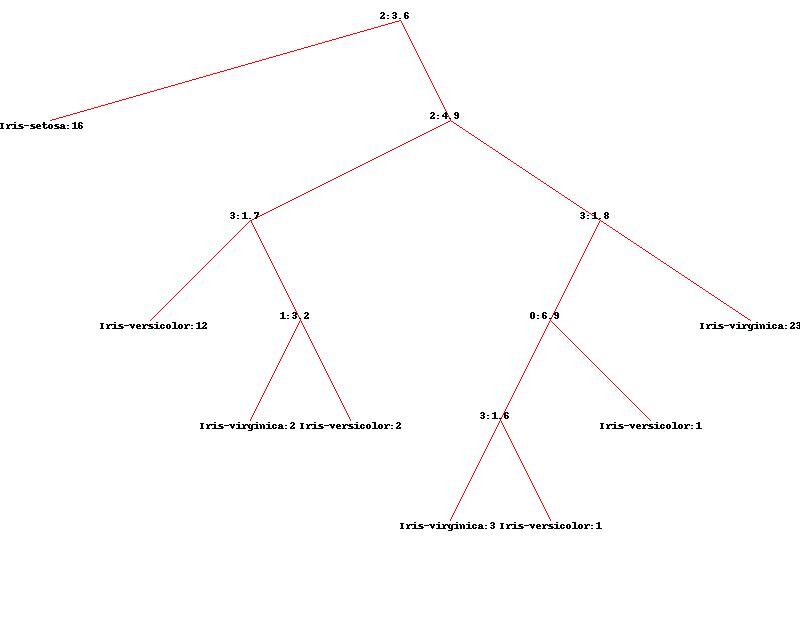
\includegraphics[scale=0.55]{iris.jpg}
		
			Otteniamo, infine, l'agognato albero di decisione!\par
			Come si evince dalla figura, il nodo scelto come radice è relativo alla terza colonna (colonna numero 2 da programma, poiché la numerazione rimarca quella delle liste in python) ed il valore che ne minimizza la funzione d'entropia è 3.6. Notiamo che questa scelta ci permette già la classificazione di 16 esempi.
			L'albero, attraverso le informazioni del training set, classifica tutti gli esempi, anche se, evidentemente, il \emph{guadagno informativo} degli attributi non sarà alto. Osserviamo, infatti, che un attributo non riesce a caratterizzare nettamente un gruppo di esempi. Conseguentemente, ciascuno di essi viene richiamato più volte per lo \emph{split} dei dati, aumentando inevitabilmente la profondità dell' albero.\par
			Alla luce di queste considerazioni, molto probabilmente questa classificazione non sarà abbastanza generalizzante ed, ipotizzando di utilizzare un test set sufficientemente vario, non ci offrirà ottimi risultati in termini di \emph{performance}. Si potrebbe, però, ricercare una maggiore generalizzazione tramite l'applicazione di tecniche di \emph{pruning}, che diminuirebbero la profondità dell'albero.\par
			%Ho tolto il fatto del rasoio di Ockam perché mi sembrava un poco forzato: si utilizza nella scelta tra più possibilità, ma in questo caso stiamo potando deliberatamente l'albero (il concetto è simile ma con una sfumatura differente)
		\subsubsection{Mushrooms} 
			Analizziamo ora il data set \emph{Muschroom}, relativo ai funghi. Il fine sarà di determinarne l' habitat. Il dataset è caratterizzato da ben 21 attributi e 8124 istanze. Utilizziamo sempre le medesime percentuali di dati per il training set ed il test set (40\%-60\%).
			
			\begin{sidewaysfigure}
				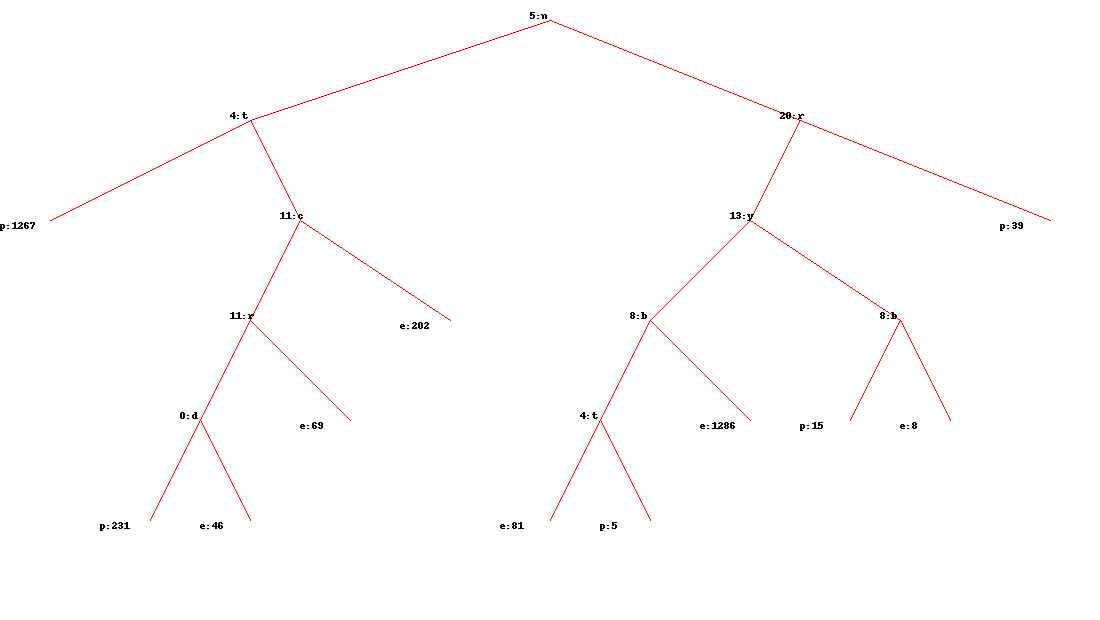
\includegraphics[width=1.2\textwidth, height=0.9\textheight]{mushroom.jpg}
				\caption{Mushrooms Decision Tree}
				\label{fig:mus-dt}
			\end{sidewaysfigure}
			
					
			L' albero, come si può osservare dalla figura \vref{fig:mus-dt}, non è in grado di classificare gli esempi distintamente. In questo stato l'albero può portare a decisioni inconcludenti. Risultato analogo si è ottenuto al seguito di differenti esperimenti sul medesimo data set, rivelandosi tutt'altro che un \textit{unicum}. Ciò ci ha portato ad interpretare questo esito come conseguenza del fatto che gli attributi utilizzati non siano abbastanza rappresentativi, non riuscendo a classificare pienamente i vari esempi.
			
		    %in seguito a vari test effettuati con diversi elementi che componevano il training set, i risultati sono appartsi sempre inconcludenti in quanto c'era sempre un numero di nodi maggiore di 3 che portavano a decisioni ambuigue, nel nodo foglia c'erano piu' risultati.Per tanto visto che stiamo studiando tale materia abbiamo deciso di soffermarci su tali risultati giungendo alle seguenti conclusioni enumerato quello che sta dopo.
		    
			Notiamo, in conclusione, che un grande numero di attributi non necessariamente porta a spiegare tutti gli esempi.
		\newpage
		\subsection{Esperimento: Learning Curve}
		In questo esempio mostreremo al variare del training set e del data set, il valore della performance dell' albero visualizzando tramite un grafico.
		Il data set che andremo ad utilizzare è stato preso da un censimento, per identificare le persone che guadagnano più di cinquanta mila dollari all' anno.
		Le righe di codice adibite alla generazione del grafico sono quelle scritte in questa funzione:
		%\vspace{2.7cm}
		\begin{python}
		def fperformance(data):
			testc=data
			percent=10
			p=[]
			perc=[]
			t=[]
			numdati=(int)((float)(len(testc))/100*percent);
			for i in range(0,5):
				(train,testc)=createdataset(testc,numdati)
				t=t+train;
				tree=buildtree(t)
				p=p+[performance(tree,testc)]
				perc=perc+[percent]
				percent=percent+10;
				line,=plt.plot(perc,p,'r-')
			plt.xlabel('percentuale dati training')
			plt.ylabel('percentuale successi')
			line.set_antialiased(False)
			plt.show()
		\end{python}
		\bigskip
	%passiamo ora a descrivere cosa fa questa funzione come prima cosa effettua una copia del dataset che gli e' stato ricevuto dopodiche' inizializza una serie di liste a supporto delle operazioni successive. farei una descrizione per linee di codice, metterei il codice per riga sia sopra che sotto commentando
		la funzione essenzialmente dopo aver fatto una copia dei dati passati,delle inizializzazioni di liste che ci occorrono per il plot dei dati e aver determinato il numero di elementi da aggiungere al training set(togliendoli al test set), iterativamente per 5 volte create data set divide i dati in train set e test set,i dati del train vengono assegnati ad una lista t che verrà usata effettivamente per il training, viene costruito l' albero, se ne calcola il valore di performance, richiamando al suo interno la funzione classify che ritorna la classificazione fatta dall ' albero con gli attributi dell' esempio e alla fine si confronta la classificazione ottenuta con il valore del test, se l' albero è riuscito a classificare bene l' esempio allora si avrà un riscontro positivo, altrimenti negativo, performance  ha come valore di ritorno la percentuale di esiti positivi sul numero di test effettuati.Dopo di che si aggiungono i punti alla linea per il plot e alla fine viene mostrata su schermo, un esempio di curva è questo:
		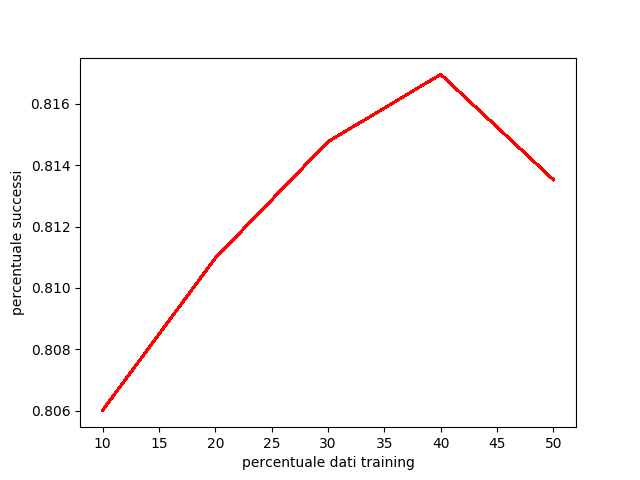
\includegraphics[scale=0.86]{performance.png}
		%evince 
		Come si vede dal grafico la nostra percentuale di apprendimento migliora fino al 40\% dopodiché si percepisce un degrado dell'apprendimento quando arriviamo al 50\% di dati utilizzati per il training-set.
		\newline
		 Su tale risultato siamo giunti alla seguente considerazione " aumentando il training-set si è costruito un albero più specifico e di conseguenza  con meno capacità di classificare gli esempi ".
		 Dalla figura che mostra l'andamento della curva di apprendimento, si intuisce che la rappresentazione dell'ambiente così descritto dai dataset è ridondante.
		  Infatti la crescita è lenta, al crescere del training-set dal 10\% al 50\% si evince che l'aumento è di circa del 1\%.
		  Per migliorare la rapidità della curva di performance dell'albero di decisione si potrebbero rimuovere alcuni attributi,se si è sicuri della rappresentazione, testando altre configurazioni dell' ambiente fino a che non vediamo miglioramenti evidenti nell' apprendimento, se ciò non avviene si può pensare di cambiare gli attributi che pensiamo essere ridondati o quelli che ci danno un basso contenuto informativo, con altri o addirittura rifare il modello dell' ambiente . 
		\subsection{Domanda 1}
		
		%tali tecniche di apprendimento mirano alla formulazione di una funzione h che approssimi la funzione f, dove ricordiamo che f è la funzione condizione azione che si vorrebbe apprendere. la costruione di h avviene 
			Un agente in grado di apprendere mediante alberi di decisione fonda questo suo processo su principi di apprendimento induttivo (\textsf{inductive learning}). L'apprendimento induttivo è una forma di apprendimento basata sull'induzione a partire da esempi dati. Esso, data una collezione di esempi (\textsf{training set}) della funzione \textsf{target} \emph{f} che si vorrebbe imparare, mira a restituire una funzione \emph{h} (\textsf{hypothesis}) che approssimi la \emph{f}, anche se non è detto che riesca a trovare una che l' approssimi bene nello spazio delle funzioni. Concettualmente, il criterio nella determinazione di \emph{h} tra le differenti funzioni dello spazio delle ipotesi dovrebbe essere legato, più che alla consistenza nello spiegare i dati, alla bontà dell'approssimazione e quindi alla capacità di generalizzazione per predire esempi non ancora incontrati. In questo senso, l'agente agisce in modo razionale poichè cerca di \textbf{decidere come comportarsi in situazioni a lui sconosciute basandosi su quelle già note}. Possiamo individuare proprio in questo aspetto una \textbf{forma di intelligenza}, determinata dall'agire razionalmente.
		\subsection{Domanda 2}
			Le procedure di \textsf{Decision Tree Learning} consentono la costruzione di un albero di decisione "piccolo", consistente con gli esempi forniti in input per la costruzione di tale struttura. Ogni nodo interno all'albero corrisponde ad una condizione sul valore di un attributo(quindi una decisione), gli archi verso i nodi figli ai possibili valori per quell'attributo(una scelta intrapresa), le foglie alla classificazione(target raggiunto). Si ottiene così, attraverso i \textsf{path} dell'albero, una rappresentazione compatta delle regole di condizione-azione. L'albero di decisione prende in input una situazione descritta da un insieme di attributi e restituisce una decisione, ovvero il valore predetto di uscita per tale input, sulla base del cammino percorso. In questo senso possiamo parlare di apprendimento, poiché, \textbf{alla luce di un dato insieme di esempi, si viene a costituire un albero di decisione dalla ben determinata topologia e legge condizione-azione, utilizzabile per la classificazione di esempi futuri}.
	\section{Esercizio 2: Problem Solving}
		\label{sec:es2}
		Il problema descritto è del tipo \emph{non deterministico} e \emph{parzialmente osservabile}, quindi classificabile come \textsf{Contingency Problem}.
		Essendo il pianeta caratterizzato da una proprietà di
		elasticità geografica, possiamo immaginare che forze esterne,
		ad ogni cambio di città del robot, facciano variare le
		distanze tra le differenti città, incrementandole o
		diminuendole. Per tale motivo l’algoritmo di navigazione
		proposto fa uso di un albero di ricerca con strategia di
		analisi in profondità (\textbf{depth-first search}), la quale
		prevede di espandere primariamente il nodo più profondo non espanso.
		%Essendo le distanze geografiche  elastiche, possiamo immaginare che forze esterne ad ogni cambio di città del robot fanno cambiare la geografia del pianeta incrementando o diminuendo le distanze tra le varie città, per tale motivo l'algoritmo di navigazione proposto fa uso di un albero di ricerca con strategia di analisi in profondità (\textsf{depth-first search}), la quale prevede di espandere primariamente il nodo più profondo non espanso.
		\newline
		 L'alterazione non deterministica delle distanze ci ha spinto a sottolineare l'importanza di \textbf{minimizzare il numero di città percorse} lungo il tragitto verso l'obiettivo. Un maggior numero di città attraversate aumenterebbe probabilisticamente la distanza percorsa. Sarebbe, quindi, auspicabile evitare, o minimizzare, il numero di processi di risalita dell'albero, che prevederebbero il ritorno alle stesse città più volte, e continuare nella navigazione in profondità, sfruttando, nel migliore dei casi, la possibilità di arrivare al \textsf{goal} senza attuare un \textsf{backtracking}.Un’ulteriore scelta, dettata dalla natura del problema, riguarda l’utilizzo
		 della struttura dati lista semplice. Ciò dipende dal fatto che, in questo
		 esempio, le distanze tra le città non sono costanti ed anzi considerate varianti
		 in maniera non predicibile e non deterministica. Quindi, la struttura dati
		 lista, ordinata in base alla distanza, non si adatta a tale tipologia di
		 problema (a differenza di quello trattato in classe).
		 Inoltre, per evitare l’insorgere di cicli, si è previsto di tenere traccia
		 dell’insieme dei nodi già esplorati mediante l’utilizzo di una lista \textsf{closed},
		 ottenendo in definitiva un algoritmo del tipo \textsf{Graph Search}. %Inoltre, per evitare l'insorgere di cicli, si è previsto di tenere traccia dell'insieme dei nodi già esplorati,mediante l'utilizzo di una lista, ottenendo in definitiva un algoritmo del tipo \textsf{Graph Search}.
%La scelta dell'utilizzo della struttura dati lista semplice, è stata dettata dalla natura del problema, in quanto a differenza del problema analogo, ma diverso trattato in classe, in questo esempio le distanze tra le città non sono costanti e quindi la struttura dati lista ordinata in base alla distanza non si adatta a tale tipologia di problema.
